\documentclass[11pt,a4paper]{article}

\usepackage[a4paper,margin=2.35cm,headheight=14pt]{geometry}
\usepackage[T1]{fontenc}
\usepackage{lmodern}
\usepackage{microtype}
\usepackage{graphicx}
\usepackage{booktabs}
\usepackage{array}
\usepackage{tabularx}
\usepackage[table]{xcolor}
\usepackage{listings}
\usepackage{caption}
\usepackage{float}
\usepackage{enumitem}
\usepackage{tikz}
\usetikzlibrary{arrows.meta,positioning,shapes.geometric}
\usepackage[hidelinks]{hyperref}

\definecolor{navy}{HTML}{163A5F}
\definecolor{lightblue}{HTML}{DCEAF7}
\definecolor{palegray}{HTML}{F3F3F3}
\definecolor{codegreen}{HTML}{2E6B32}
\definecolor{codeblue}{HTML}{1F4E79}

\makeatletter
\def\ps@assignment{%
  \def\@oddhead{%
    \vbox{\hbox to\textwidth{\small Embedded Real Time Systems -- Assignment 2\hfil\thepage}%
    \vskip2pt\hrule}}%
  \let\@evenhead\@oddhead
  \def\@oddfoot{}%
  \let\@evenfoot\@oddfoot}
\let\ps@plain\ps@assignment
\makeatother
\pagestyle{assignment}

\setlength{\parindent}{0pt}
\setlength{\parskip}{0.6em}
\widowpenalty=10000
\clubpenalty=10000
\setcounter{tocdepth}{2}
\renewcommand{\arraystretch}{1.2}

\lstdefinestyle{cppstyle}{
  language=C++,
  basicstyle=\ttfamily\small,
  keywordstyle=\color{codeblue}\bfseries,
  commentstyle=\color{codegreen},
  stringstyle=\color{purple},
  numbers=left,
  numberstyle=\tiny\color{gray},
  stepnumber=1,
  numbersep=8pt,
  frame=single,
  rulecolor=\color{gray!35},
  backgroundcolor=\color{palegray},
  breaklines=true,
  showstringspaces=false,
  tabsize=4,
  columns=fullflexible,
  keepspaces=true,
  xleftmargin=1.5em,
  framexleftmargin=1.2em
}

\newcommand{\statuspending}{\textit{Physical board evidence pending walkthrough.}}

\title{%
  \textbf{Embedded Real Time Systems}\\[0.5em]
  Assignment 2 -- Building SoPC Designs on the ZYBO FPGA Platform}
\author{%
  \begin{tabular}{ll}
  Student Name & Student ID \\
  \hline
  Firas Harbo Saleh & 202109174
  \end{tabular}}
\date{11 October 2026}

\begin{document}

\maketitle

\section*{Introduction}
This journal documents the mandatory exercises 3, 4, 5, and 7 from Assignment 2
in Embedded Real Time Systems. The work progresses from bare-metal control on the
Zynq processing system to custom acceleration in programmable logic. The
implementation includes a UART command interpreter, GPIO and timer control,
software and hardware matrix multiplication, and a fixed-point neural network
implemented with High Level Synthesis.

The software matrix implementation and the neural-network C model were verified
with self-checking tests. The neural-network design was synthesized for the
XC7Z010, passed VHDL C/RTL co-simulation, was implemented in Vivado 2026.1, and
was executed on the ZYBO as a native Cortex-A9 application built by Vitis 2026.1.
All ten accelerator outputs matched the software reference. The application
screenshots are direct captures from the earlier native session on 10 October,
retained as historical views of the tools. The updated measurements use raw
UART and build logs from 11 October, not reconstructed screenshots.

The course specifies 2017.2; acceptance of 2026.1 is not yet established.
The original ANN testbench and the documented adapted fixed-point reference
also differ, as explained in the verification section. These boundaries prevent
an unqualified claim that every written acceptance condition is complete.

\begin{table}[H]
\centering
\caption{Implementation and verification overview}
\small
\begin{tabularx}{\textwidth}{>{\centering\arraybackslash}p{1.7cm} p{5.1cm} X}
\toprule
\textbf{Exercise} & \textbf{Implementation} & \textbf{Verification state} \\
\midrule
3 & UART, custom LED IP, timer, OCM & Native build/UART passed; user observed full LED counter \\
4 & $4\times4$ software matrix multiplication & Host and native ZYBO result passed \\
5 & AXI matrix accelerator integration & Three native software/hardware comparisons passed \\
7 & Fixed-point ANN in HLS and Vitis & Adapted-model verification; original-reference acceptance remains open \\
\bottomrule
\end{tabularx}
\end{table}

\clearpage
\tableofcontents
\clearpage

\section{Exercise 3: UART Console Application}

\subsection{Task}
The application must implement a command language controlled through USB-UART.
Command \texttt{1} reads switches SW0--SW3 and displays the four-bit value on
LED0--LED3. Command \texttt{2} presents a binary counter on the LEDs and advances
once per second.

\subsection{Design}
The switches use AXI GPIO configured as input. The supplied custom LED IP is
controlled by a write to its register 0; it is not an AXI GPIO device. The
generated address map supplies each peripheral address. Under the modern SDT
driver flow GPIO initialization uses its base address; a separate legacy path
retains SDK device-ID lookup. The Cortex A9 private SCU timer supplies the delay.
The timer runs at half of the 650 MHz processor clock, so a one-second interval is
represented by 325,000,000 timer ticks. A line-oriented parser accepts complete
commands and reports invalid input rather than silently ignoring it.

\begin{lstlisting}[style=cppstyle,caption={UART command dispatch}]
if (strcmp(command, "1") == 0) {
    copySwitches();
} else if (strcmp(command, "2") == 0) {
    runCounter();
} else if (strcmp(command, "help") == 0) {
    showHelp();
} else {
    xil_printf("Unknown command '%s'.\r\n", command);
}
\end{lstlisting}

The switch command masks the read value to four bits before writing it to the
custom LED register. This prevents unrelated bits from affecting the result.

\begin{lstlisting}[style=cppstyle,caption={Switch-to-LED transfer}]
const u32 value = XGpio_DiscreteRead(&switches, GPIO_CHANNEL)
                  & LED_MASK;
Xil_Out32(ERTS_LED_BASEADDR, value);
xil_printf("Switch value: 0x%x\r\n", value);
\end{lstlisting}

The counter writes all sixteen possible four-bit patterns. Polling the timer is
appropriate here because the exercise intentionally demonstrates basic
bare-metal control and no other task must execute concurrently.

\begin{lstlisting}[style=cppstyle,caption={One-second binary LED counter}]
// Timer is started once with auto-reload at 325,000,000 ticks.
for (value = 0U; value <= LED_MASK; ++value) {
    setLeds(value);
    xil_printf("Counter: %d\r\n", value);
    if (value != LED_MASK) {
        while (!XScuTimer_IsExpired(&timer.instance)) {}
        XScuTimer_ClearInterruptStatus(&timer.instance);
    }
}
// Stop the timer and disable auto-reload after the final value.
\end{lstlisting}

\subsection{Native Build and Physical Result}
The application was built with Vitis 2026.1 at \texttt{-O2} on the supplied
Ex5 platform reconstructed for 2026.1. It retains the Ex3 processor, switches
and custom LEDs while also providing the matrix IP used by Exercise 5.
The selected linker script puts the heap at \texttt{0x1000--0x2FFF} and all
stack modes at \texttt{0x3000--0x67FF}; inspection of the actual ARM ELF verifies
these OCM ranges and retention of the SDT driver configuration section.

Real UART returned switch value \texttt{0xF}, every counter value 0--15, and the
correct matrix result for the added \texttt{mult} command. Host UART arrival
intervals on the first run were approximately 0.992--1.008 seconds; USB scheduling
introduces jitter. During the requested rerun, the user confirmed: ``Yes, the
full count looked correct'' in response to observing all four LEDs from 0000
to 1111 at about one step per second. This is physical user observation,
not a camera recording. A separate switch-by-switch mapping test remains pending.

\section{Exercise 4: Software Matrix Multiplication}

\subsection{Task and Data Representation}
Three global arrays named \texttt{aInst}, \texttt{bTInst}, and \texttt{pInst}
store matrix $A$, the transpose of matrix $B$, and the product $P$. Each row uses
a union named \texttt{vectorType}; \texttt{VectorArray} is an array of four rows.
The component view is convenient for software,
while the packed 32-bit view is reused by the hardware accelerator in Exercise 5.

\begin{lstlisting}[style=cppstyle,caption={Packed matrix row}]
typedef union {
    unsigned char comp[MSIZE];
    unsigned int vect;
} vectorType;
typedef vectorType VectorArray[MSIZE];

void setInputMatrices(VectorArray A, VectorArray B);
void displayMatrix(VectorArray input);
void multiMatrixSoft(VectorArray A, VectorArray B, VectorArray P);
void multiMatrixHard(VectorArray A, VectorArray B, VectorArray P);
\end{lstlisting}

\begin{table}[H]
\centering
\caption{Input matrices and expected product}
\begin{tabular}{c cccc c cccc c cccc}
\toprule
& \multicolumn{4}{c}{$A$} && \multicolumn{4}{c}{$C$ (stored $B^T$)} && \multicolumn{4}{c}{$P=A C^T$} \\
\cmidrule{2-5}\cmidrule{7-10}\cmidrule{12-15}
0 & 1&2&3&4 && 1&2&3&4 && 30&30&30&30 \\
1 & 5&6&7&8 && 1&2&3&4 && 70&70&70&70 \\
2 & 9&10&11&12 && 1&2&3&4 && 110&110&110&110 \\
3 & 13&14&15&16 && 1&2&3&4 && 150&150&150&150 \\
\bottomrule
\end{tabular}
\end{table}

\subsection{Implementation}
The stored layout follows the literal transpose printed on assignment p.~6.
Writing $C$ for the stored array avoids ambiguity: the operation is
$P_{ij}=\sum_k A_{ik}C_{jk}\pmod{256}$. The previous constant-row input
layout remains a separate regression test, not the submitted fixture.

For every output element, the algorithm calculates the dot product of one row
from $A$ and one row from the stored transpose of $B$. The three nested loops
perform $4\times4\times4=64$ byte multiplications.

\begin{lstlisting}[style=cppstyle,caption={Software matrix multiplication}]
for (row = 0; row < MSIZE; ++row) {
    for (col = 0; col < MSIZE; ++col) {
        unsigned int sum = 0U;
        for (k = 0; k < MSIZE; ++k) {
            sum += (unsigned int)A[row].comp[k] * B[col].comp[k];
        }
        P[row].comp[col] = (unsigned char)sum;
    }
}
\end{lstlisting}

The command \texttt{mult} initializes the matrices, starts the SCU timer, calls
the software multiplication, stops the timer, and prints all three matrices and
the elapsed tick count to USB-UART.

\subsection{Verification}
A host-side unit test compares all sixteen calculated elements with the expected
product in Table 2. The expanded suite covers the course transpose, the previous
fixture, non-symmetric rows and modulo-256 overflow; all pass. The standalone
Ex4 application returned the same matrix on the ZYBO and measured 260 SCU timer
ticks, or 0.800 $\mu$s at 325 MHz. This is one observed \texttt{-O2} run, not
a statistical CPU benchmark.

The reproducible host command is
\texttt{make -C Assignment\_2 test}; it exits successfully after printing
\texttt{matrix test: PASS}.

\section{Exercise 5: Hardware Matrix Accelerator}

\subsection{Hardware and Software Partition}
The custom matrix IP replaces the inner software loop. The processor writes one
packed row from $A$ to AXI register 0 and one packed row from $B^T$ to AXI
register 1. Programmable logic performs four parallel eight-bit products, adds
the partial results, and exposes the dot product in register 2.

\begin{figure}[H]
\centering
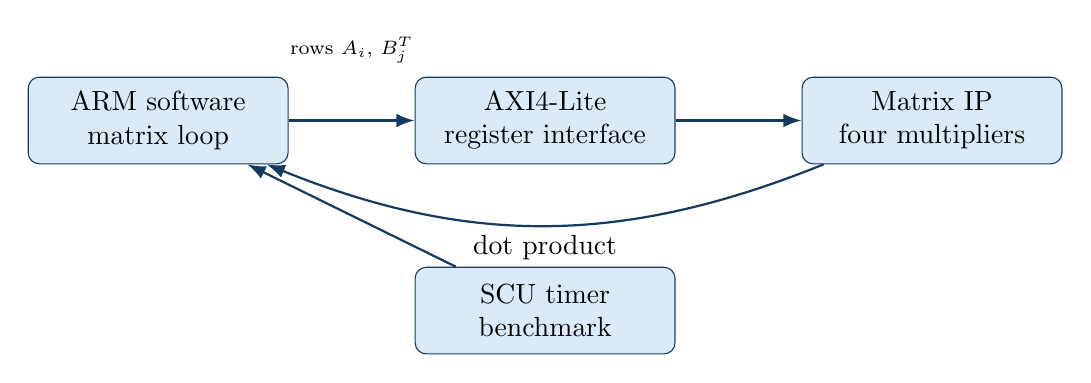
\begin{tikzpicture}[
  node distance=13mm and 16mm,
  block/.style={draw=navy,rounded corners,fill=lightblue,minimum width=33mm,
                minimum height=11mm,align=center},
  arrow/.style={-Latex,thick,draw=navy}]
\node[block] (sw) {ARM software\\matrix loop};
\node[block,right=of sw] (axi) {AXI4-Lite\\register interface};
\node[block,right=of axi] (ip) {Matrix IP\\four multipliers};
\node[block,below=of axi] (timer) {SCU timer\\benchmark};
\draw[arrow] (sw) -- node[above=6mm,font=\scriptsize]{rows $A_i$, $B_j^T$} (axi);
\draw[arrow] (axi) -- (ip);
\draw[arrow] (ip) to[bend left=22] node[below]{dot product} (sw);
\draw[arrow] (timer) -- (sw);
\end{tikzpicture}
\caption{Matrix accelerator data path}
\end{figure}

\begin{minipage}{\textwidth}
\begin{lstlisting}[style=cppstyle,caption={Memory-mapped accelerator access}]
Xil_Out32(BASE + REG0_OFFSET, a[row].vect);
Xil_Out32(BASE + REG1_OFFSET, bT[col].vect);
product[row].comp[col] =
    (uint8_t)Xil_In32(BASE + REG2_OFFSET);
\end{lstlisting}
\end{minipage}

\subsection{Benchmark Method}
The application measures both implementations with identical inputs. The
software interval contains all 64 processor multiplications. The hardware
interval contains sixteen accelerator calls, including two AXI writes and one
AXI read for each output. Finally, all sixteen hardware outputs are compared
with the software reference.

\begin{table}[H]
\centering
\caption{Exercise 5 native ZYBO measurements, application \texttt{-O2}}
\begin{tabularx}{\textwidth}{p{3.0cm} X X}
\toprule
\textbf{Run} & \textbf{Software ticks / time} & \textbf{Hardware ticks / time} \\
\midrule
First & 264 / 0.812 $\mu$s & 3,190 / 9.815 $\mu$s \\
Second & 197 / 0.606 $\mu$s & 3,116 / 9.588 $\mu$s \\
Third & 192 / 0.591 $\mu$s & 3,122 / 9.606 $\mu$s \\
\bottomrule
\end{tabularx}
\end{table}

\subsection{Discussion}
The exercise exposes the central tradeoff in acceleration. Parallel arithmetic
reduces computation latency, but memory-mapped communication adds overhead. For
this small matrix, AXI transfers may dominate. Larger workloads, batching,
streaming, or local buffering would amortize the transfer cost more effectively.
All three runs returned \texttt{Verification: PASS}; the capture also checked
both output matrices against the independently known literal-transpose result.
The 650 MHz ARM executes this small optimized loop faster than sixteen sets of
AXI register transfers to the 100 MHz PL. Timer overhead is included and is not
subtracted; first-run cache effects and limited sample count qualify the figures.

The Ex345 implementation met timing with WNS $+1.216$ ns, WHS $+0.046$ ns,
zero negative slack and zero final DRC violations. Original board DDR preset
skew warnings were retained during BD validation; the generated native apps
subsequently ran successfully on this board.

\section{Exercise 7: HLS Neural Network Accelerator}

\subsection{Network Structure}
The accelerator implements a fully connected network with 196 signed eight-bit
inputs, 32 hidden neurons, and 10 outputs. Input and output weights are signed
16-bit Q15 values. Each dot-product accumulator is shifted right by 15 bits to
restore the numeric scale. Negative hidden-layer values are replaced by zero
with a ReLU activation function.

\begin{table}[H]
\centering
\caption{Neural-network parameters}
\begin{tabularx}{\textwidth}{p{3.1cm} p{2.3cm} X}
\toprule
\textbf{Parameter} & \textbf{Value} & \textbf{Meaning} \\
\midrule
\texttt{INPUT\_LEN} & 196 & Downsampled image input values \\
\texttt{NEURONS\_LEN} & 32 & Hidden-layer neurons \\
\texttt{OUTPUT\_LEN} & 10 & Output classes \\
\texttt{BITS} & 15 & Fractional weight bits \\
Weight arrays & AXI4-Lite & Processor-controlled memories \\
Switch and LED ports & 4 bits & Direct pass-through demonstration \\
\bottomrule
\end{tabularx}
\end{table}

\subsection{Fixed-Point Implementation}
Weights are stored neuron-major. Each hidden neuron consumes a contiguous block
of 196 input weights, and each output consumes 32 output weights. The indexing is
important: using the number of neurons rather than the input length as the first
stride would mix weights between neurons.

\begin{lstlisting}[style=cppstyle,caption={Hidden and output layer calculations}]
accumulator += (ap_int<8>)input[j]
               * (ap_int<16>)weightsI[i * INPUT_LEN + j];
neuron = (int)(accumulator >> BITS);
neurons[i] = neuron > 0 ? neuron : 0;

accumulator += (ap_int<32>)neurons[j]
               * (ap_int<16>)weightsO[i * NEURONS_LEN + j];
output[i] = (int)(accumulator >> BITS);
\end{lstlisting}

The arrays are mapped to AXI4-Lite interfaces. The switches and LEDs use direct
ports so that the synthesized IP can demonstrate a visible hardware connection.

\begin{lstlisting}[style=cppstyle,caption={HLS interface directives}]
#pragma HLS INTERFACE ap_none port=inSwitch
#pragma HLS INTERFACE ap_none port=outLeds
#pragma HLS INTERFACE s_axilite port=input bundle=BUS
#pragma HLS INTERFACE s_axilite port=weightsI bundle=BUS
#pragma HLS INTERFACE s_axilite port=weightsO bundle=BUS
#pragma HLS INTERFACE s_axilite port=output bundle=BUS
#pragma HLS INTERFACE s_axilite port=return bundle=BUS
\end{lstlisting}

\subsection{Testbench}
An independent 64-bit fixed-point reference traverses each weight array in
sequence and implements floor division explicitly for negative Q15 values.
Five cases cover the adapted course vector, bounded signed values, zero input
after a nonzero inference, negative hidden activations, and signed extremes.
Every case checks all outputs and the switch/LED port value. An additional
8/3/4-dimension configuration is checked on the host, not on the FPGA.

The original course testbench is preserved unchanged under
\path{hls/provided_course/}. It uses overlapping weight-row strides and a
floating-point reference; all ten comparisons fail against the contiguous
fixed-point model. The adapted course test retains the supplied data generation
but corrects those reference assumptions. This documented deviation still
requires course acceptance; passing the adapted test is not passing the
untouched original.

The C-simulation transcript is stored with the HLS project and ends with
\texttt{neural network test: PASS}. The independent reference calculation makes
this a functional check rather than a comparison against copied accelerator
code.

\subsection{Baseline and Pipelined Synthesis}
Two solutions were synthesized for \texttt{xc7z010clg400-1} with a 10 ns target
clock. The baseline disables automatic loop pipelining. The optimized solution
applies initiation interval 1 directives to both inner dot-product loops.

\begin{figure}[H]
\centering
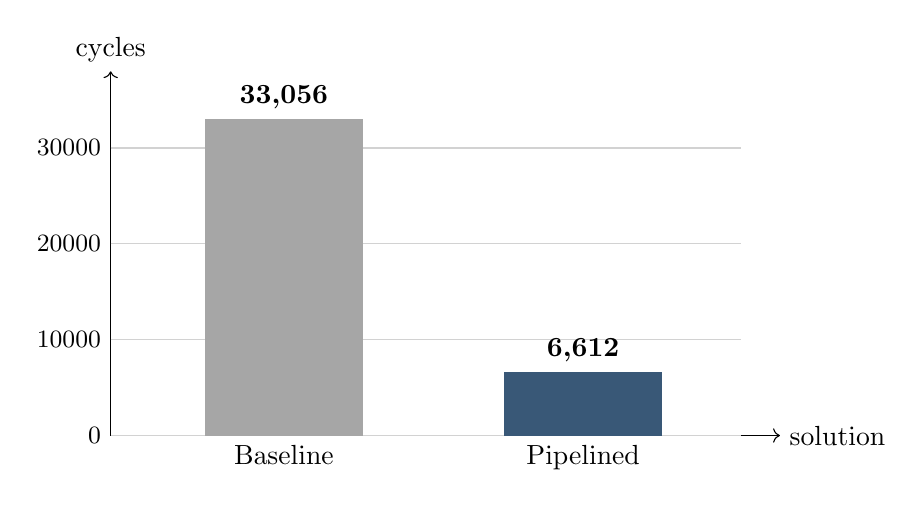
\begin{tikzpicture}[x=1cm,y=0.00012cm]
  \draw[->] (0,0) -- (8.5,0) node[right]{solution};
  \draw[->] (0,0) -- (0,38000) node[above]{cycles};
  \foreach \y in {0,10000,20000,30000} {
    \draw[gray!35] (0,\y) -- (8,\y);
    \node[left] at (0,\y) {\small\y};
  }
  \fill[gray!70] (1.2,0) rectangle (3.2,33056);
  \fill[navy!85] (5.0,0) rectangle (7.0,6612);
  \node[above] at (2.2,33056) {\textbf{33,056}};
  \node[above] at (6.0,6612) {\textbf{6,612}};
  \node[below] at (2.2,0) {Baseline};
  \node[below] at (6.0,0) {Pipelined};
\end{tikzpicture}
\caption{Estimated neural-network latency}
\end{figure}

\begin{table}[H]
\centering
\caption{HLS synthesis comparison}
\begin{tabular}{lrrrrr}
\toprule
\textbf{Solution} & \textbf{Latency} & \textbf{BRAM 18K} & \textbf{DSP} & \textbf{FF} & \textbf{LUT} \\
\midrule
Baseline & 33,056 & 10 & 2 & 638 & 716 \\
Pipelined, II=1 & 6,612 & 10 & 3 & 1,112 & 1,126 \\
\bottomrule
\end{tabular}
\end{table}

Pipelining reduces estimated latency by approximately five times. The optimized
solution uses one additional DSP, 474 additional flip-flops, and 410 additional
lookup tables; BRAM usage is unchanged. The tool estimated a maximum frequency
of approximately 194 MHz for the baseline and 143 MHz for the pipelined solution,
both above the 100 MHz target constraint.

\subsection{C/RTL Co-Simulation and Export}
The optimized VHDL solution passed C/RTL co-simulation for all five test cases,
including the adapted course vector. Reported latency was 6,610 / 6,612 / 6,613
cycles (minimum / average / maximum). The testbench transaction intervals include
AXI stimulus/loading gaps and are not the II=1 inner-loop initiation interval.
Post-checking confirmed every output and LED-port result. The core was
exported as VHDL IP version 1.0.1 as required by the assignment.

The supplied Exercise 7 Vivado project was migrated from its legacy format to
Vivado 2026.1. The regenerated HLS IP was connected through two AXI4-Lite
interfaces, the renamed switch and LED ports were repaired, and explicit ZYBO
pin constraints were applied. Implementation completed without routing errors
and met timing with 3.462 ns worst slack and zero total negative slack.

\begin{figure}[H]
\centering
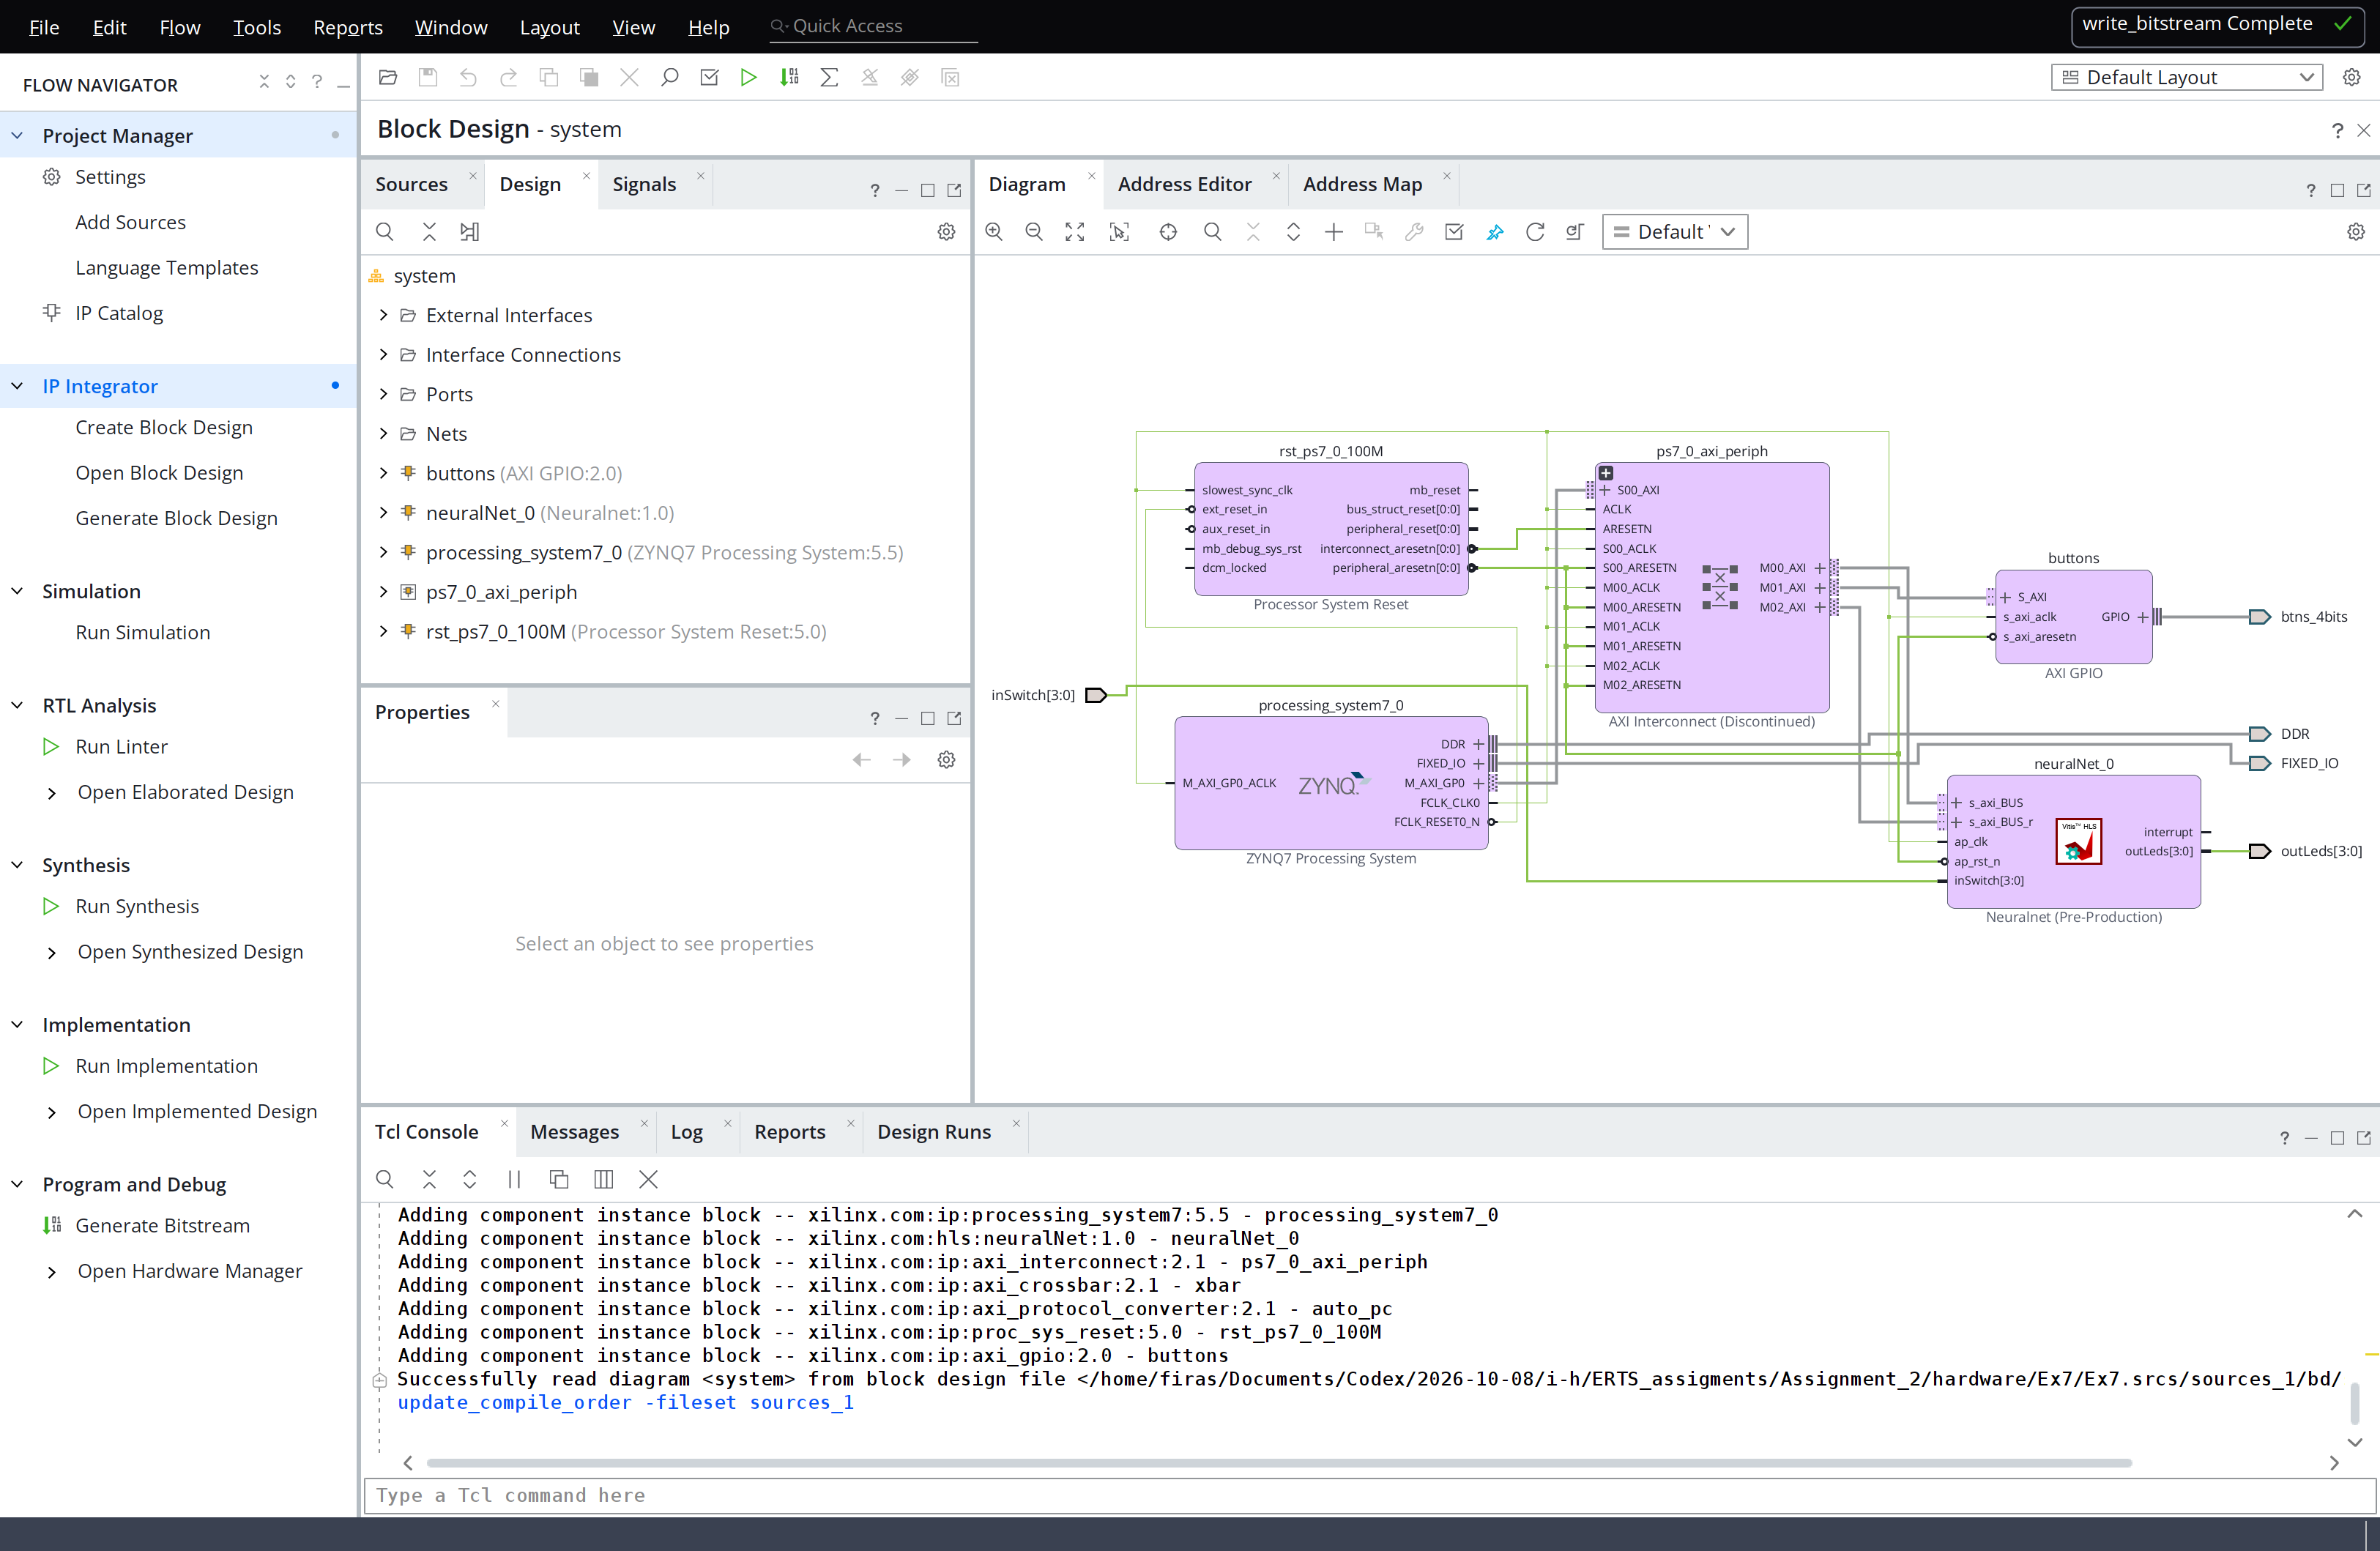
\includegraphics[width=\textwidth]{native_screenshots/vivado_ex7_block_design.png}
\caption{Historical native capture (10 October): Exercise 7 block design in Vivado 2026.1}
\end{figure}

The implemented design uses 959 LUTs, 1,097 flip-flops, six BRAM tiles, and
three DSP slices. Figure~\ref{fig:vivado-summary} shows the completed native
implementation run and its timing and utilization summaries.

\begin{figure}[H]
\centering
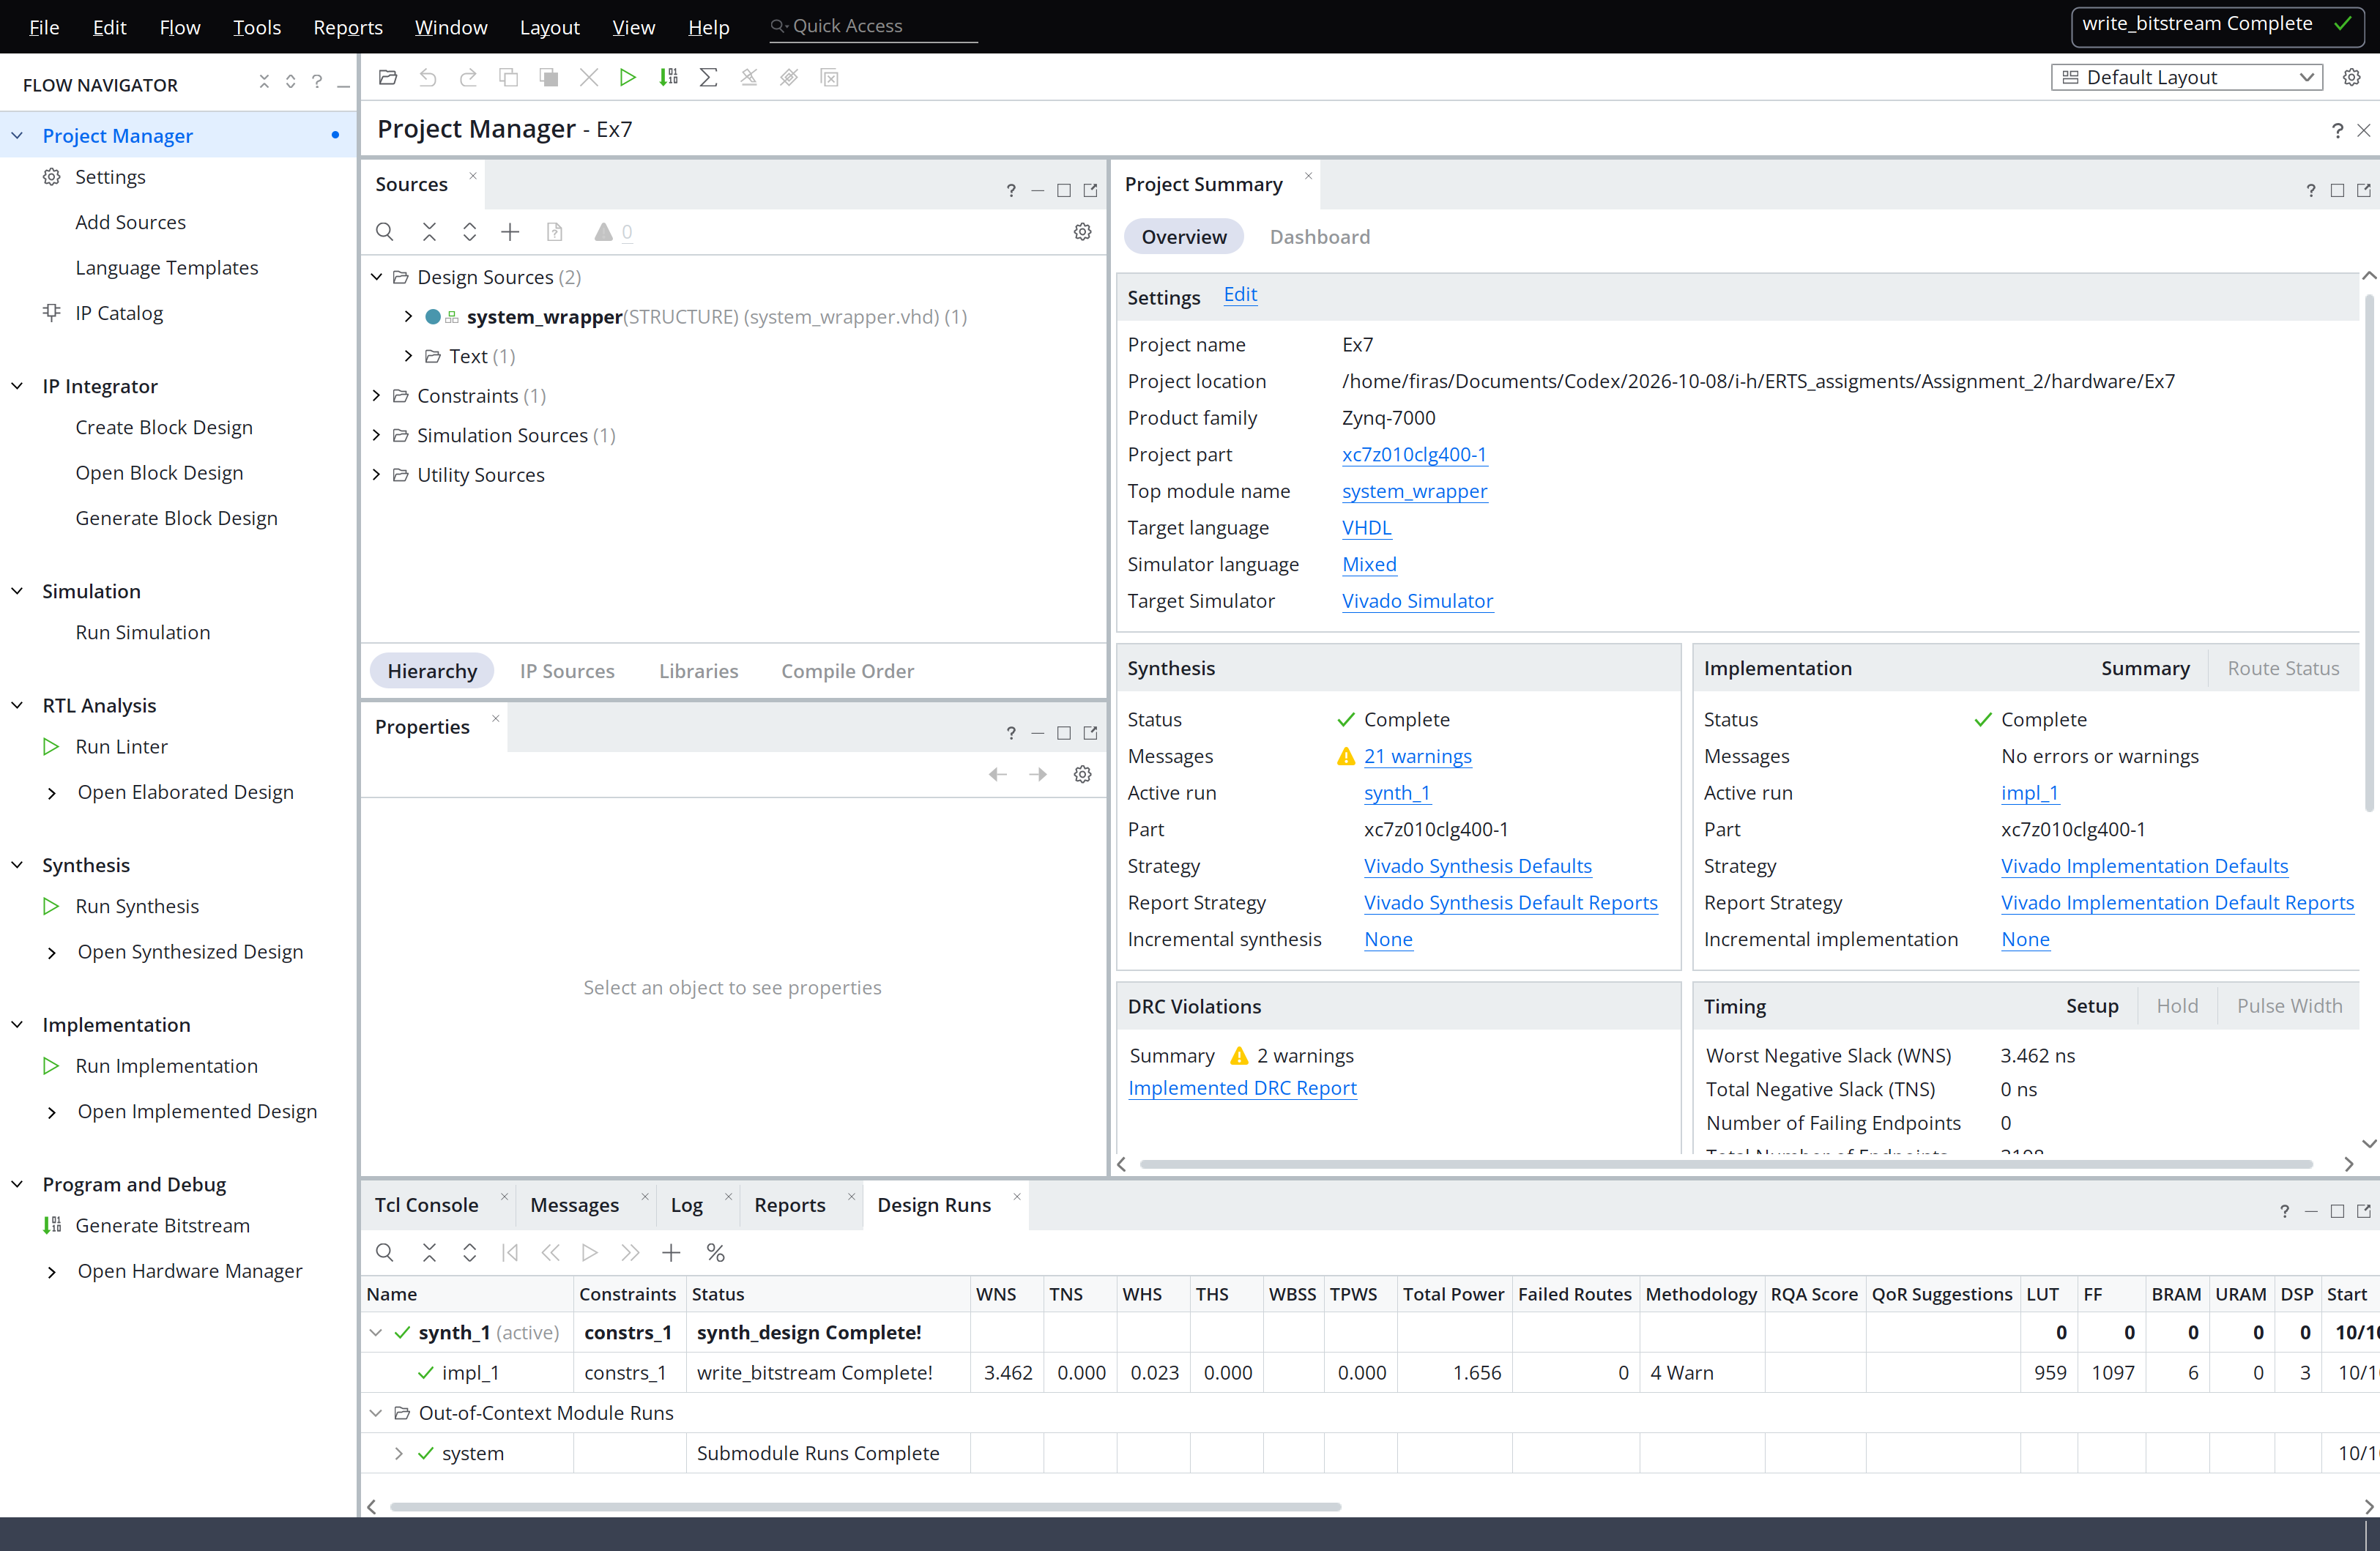
\includegraphics[width=\textwidth]{native_screenshots/vivado_ex7_project.png}
\caption{Historical native capture (10 October): completed Vivado project summary}
\label{fig:vivado-summary}
\end{figure}

The generated bitstream was programmed through the Digilent JTAG target. A
Hardware Manager refresh returned DONE status 1 for \texttt{xc7z010\_1}.

\begin{figure}[H]
\centering
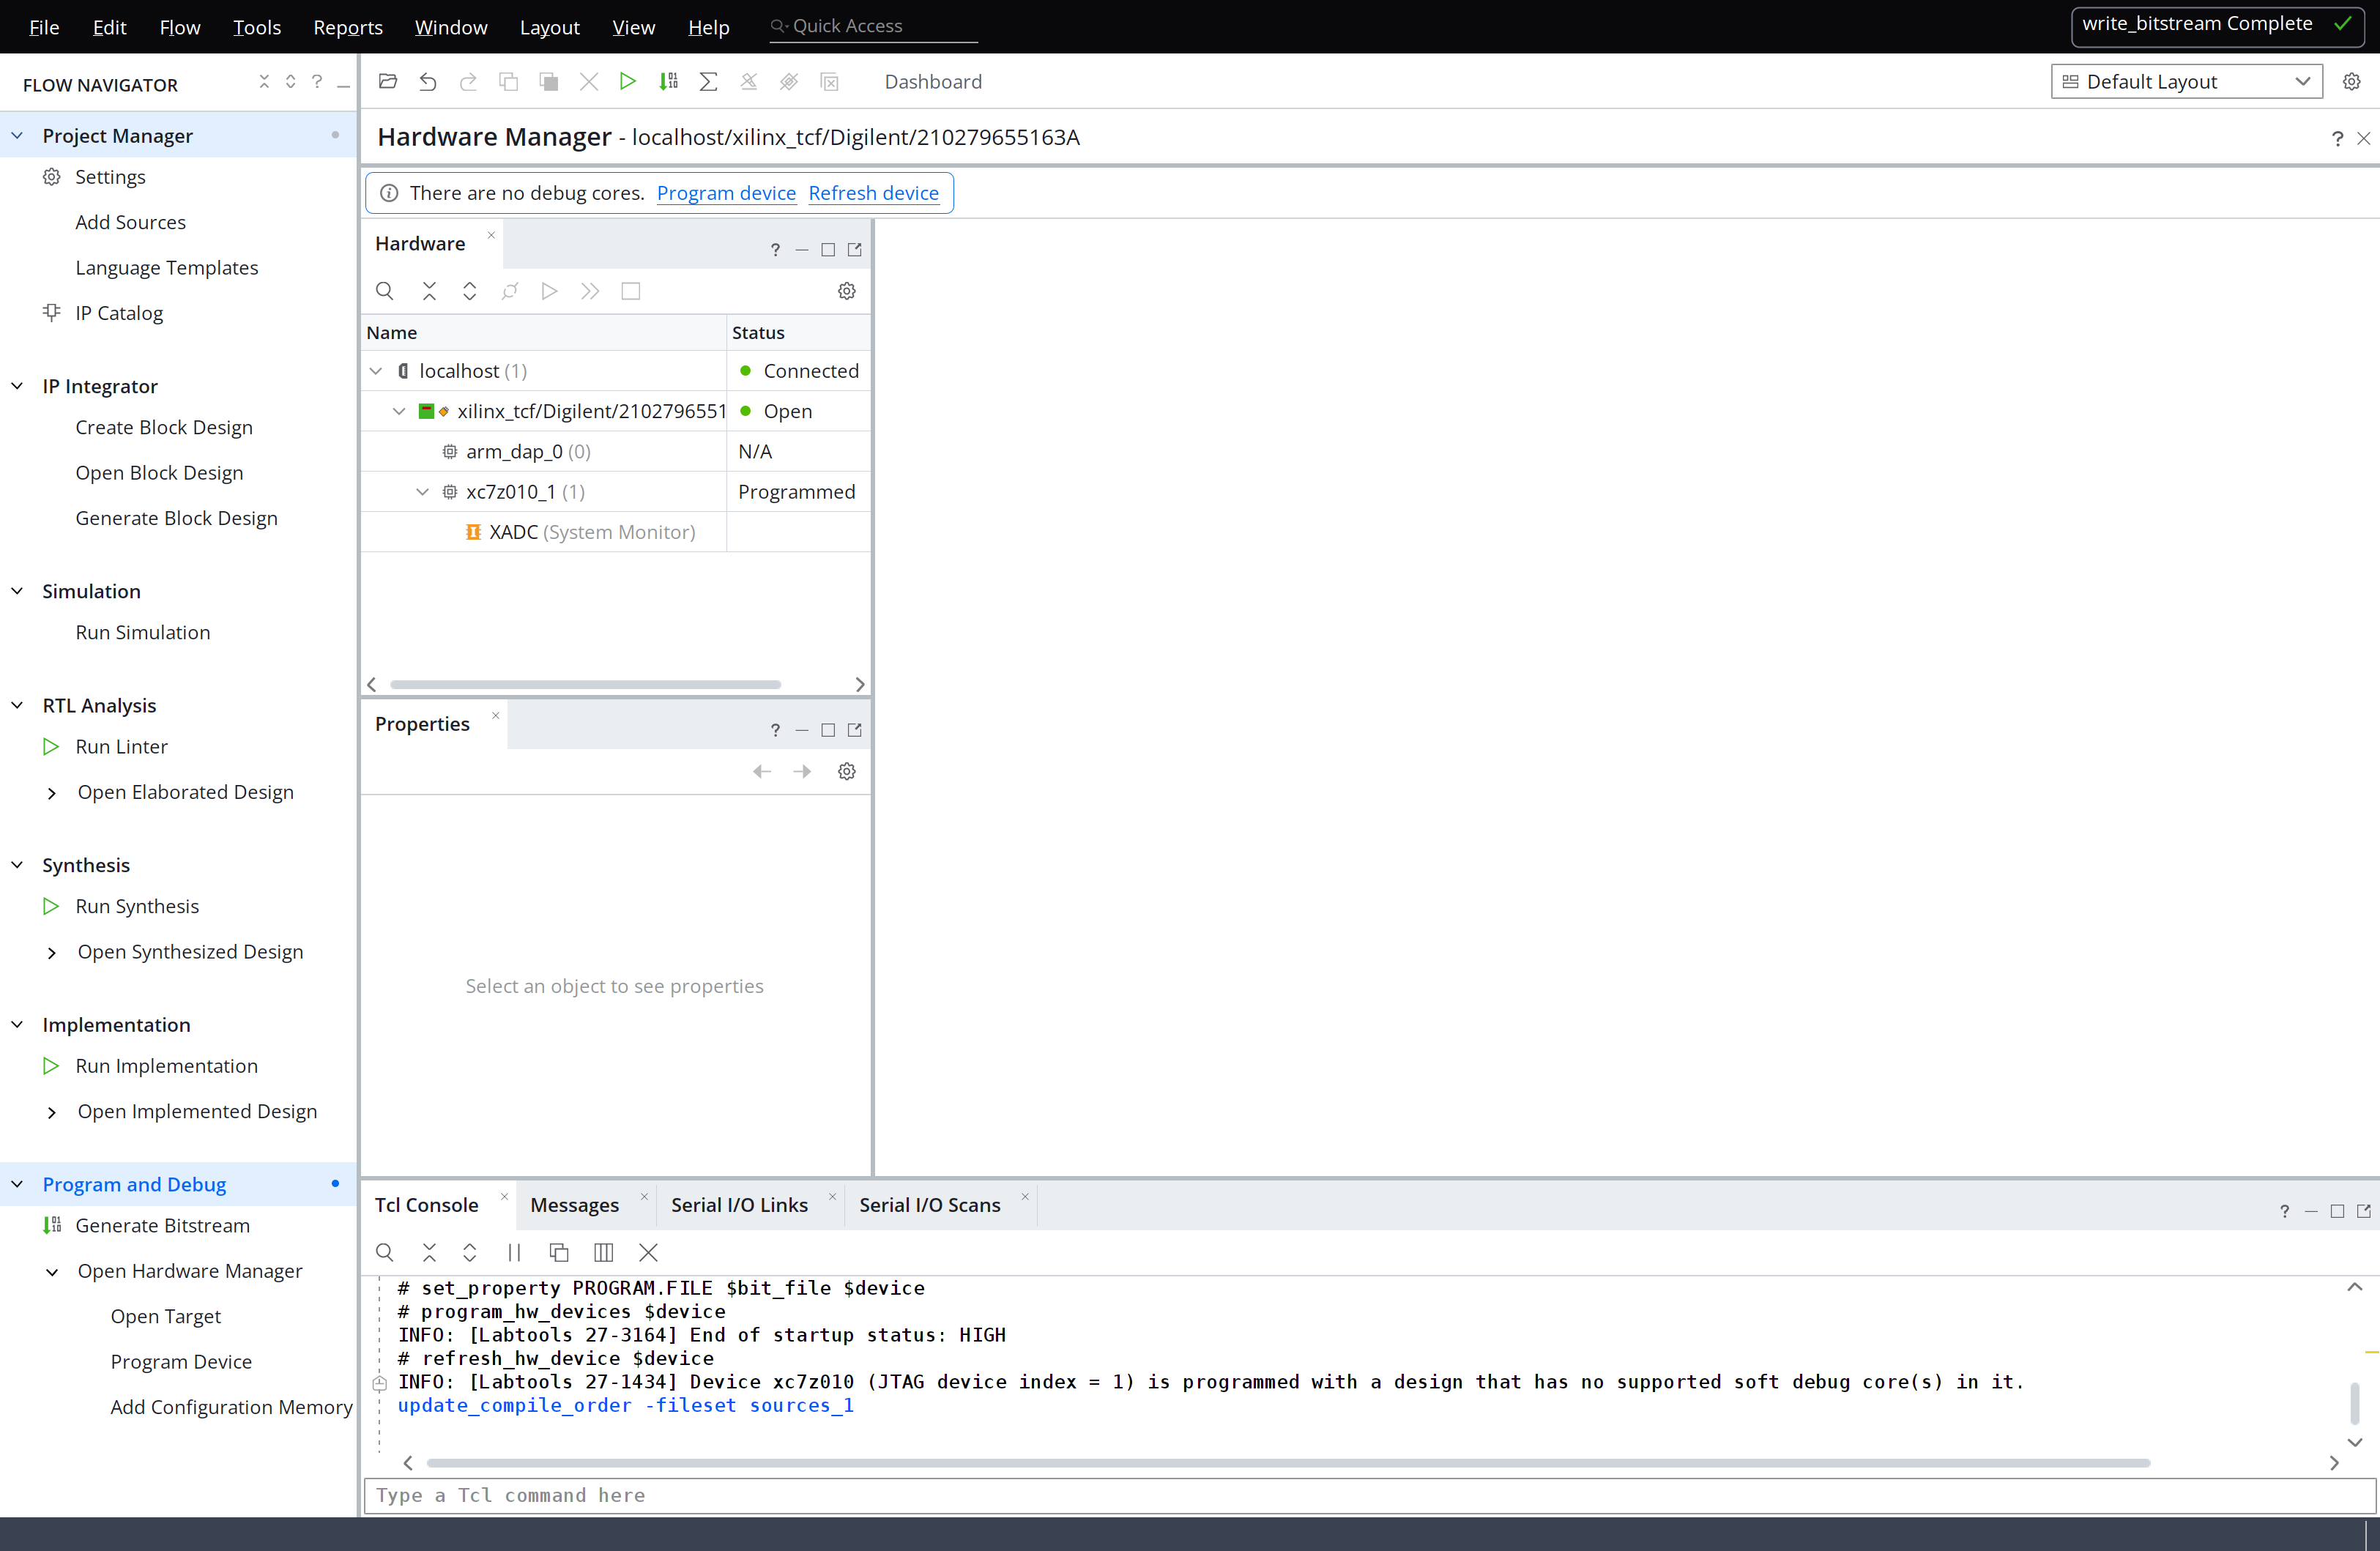
\includegraphics[width=\textwidth]{native_screenshots/vivado_hardware_manager_programmed.png}
\caption{Historical native capture (10 October): Hardware Manager with ZYBO programmed}
\end{figure}

\subsection{Vitis Integration and Target Benchmark}
The Vitis application evaluates the network in software, transfers the input and
both weight arrays through AXI, starts the accelerator, waits for completion,
and reads ten outputs. CPU timing is separate; one continuous hardware timer
measures the full transaction, with snapshots for loading and start-to-done.
The native compiler command is verified as \texttt{-O2 -g3}.

\begin{table}[H]
\centering
\caption{Exercise 7: ten subsequent verified trials at \texttt{-O2}}
\small
\begin{tabular}{lrrrr}
\toprule
\textbf{Measurement} & \textbf{Min ticks} & \textbf{Mean ticks} & \textbf{Max ticks} & \textbf{Mean time} \\
\midrule
CPU compute & 13,844 & 14,373 & 14,757 & 44.2 $\mu$s \\
HW data loading & 228,396 & 228,451 & 228,567 & 702.9 $\mu$s \\
HW start-to-done & 21,623 & 21,632 & 21,636 & 66.6 $\mu$s \\
HW FULL transaction & 253,315 & 253,386 & 253,559 & 779.6 $\mu$s \\
\bottomrule
\end{tabular}
\end{table}

The 325 MHz SCU timer reports integer-mean ticks. The separate first-run
CPU/load/run/FULL values were 14,789 / 233,803 / 21,648 / 259,189 ticks.
FULL includes packing, all input/weight writes, readiness, execution, output
readback and unpacking. It excludes platform setup, creation of test data,
verification and UART output. Timer/snapshot overhead is included.

With optimization enabled, the ARM reference is approximately $1.51\times$
faster than accelerator computation alone; the full hardware transaction is
$17.63\times$ slower than CPU compute. This supersedes the earlier $8.61\times$
claim against an unoptimized \texttt{-O0} reference. Loading dominates the
hardware path, and the 100 MHz core is not faster than the 650 MHz optimized
ARM loop for this vector. The $5\times$ HLS baseline-to-pipeline improvement is
a different, still valid comparison.

All ten outputs matched on the initial and ten repeated transactions using
the same custom signed vector and enabled caches. This is not a broad
performance characterization or board execution of every HLS test vector.
The fresh compiler/UART evidence is retained under \path{outputs/fix_evidence/}.
Figure~\ref{fig:vitis-build} is the earlier native workspace capture, not proof
of the new compiler flags.

\begin{figure}[H]
\centering
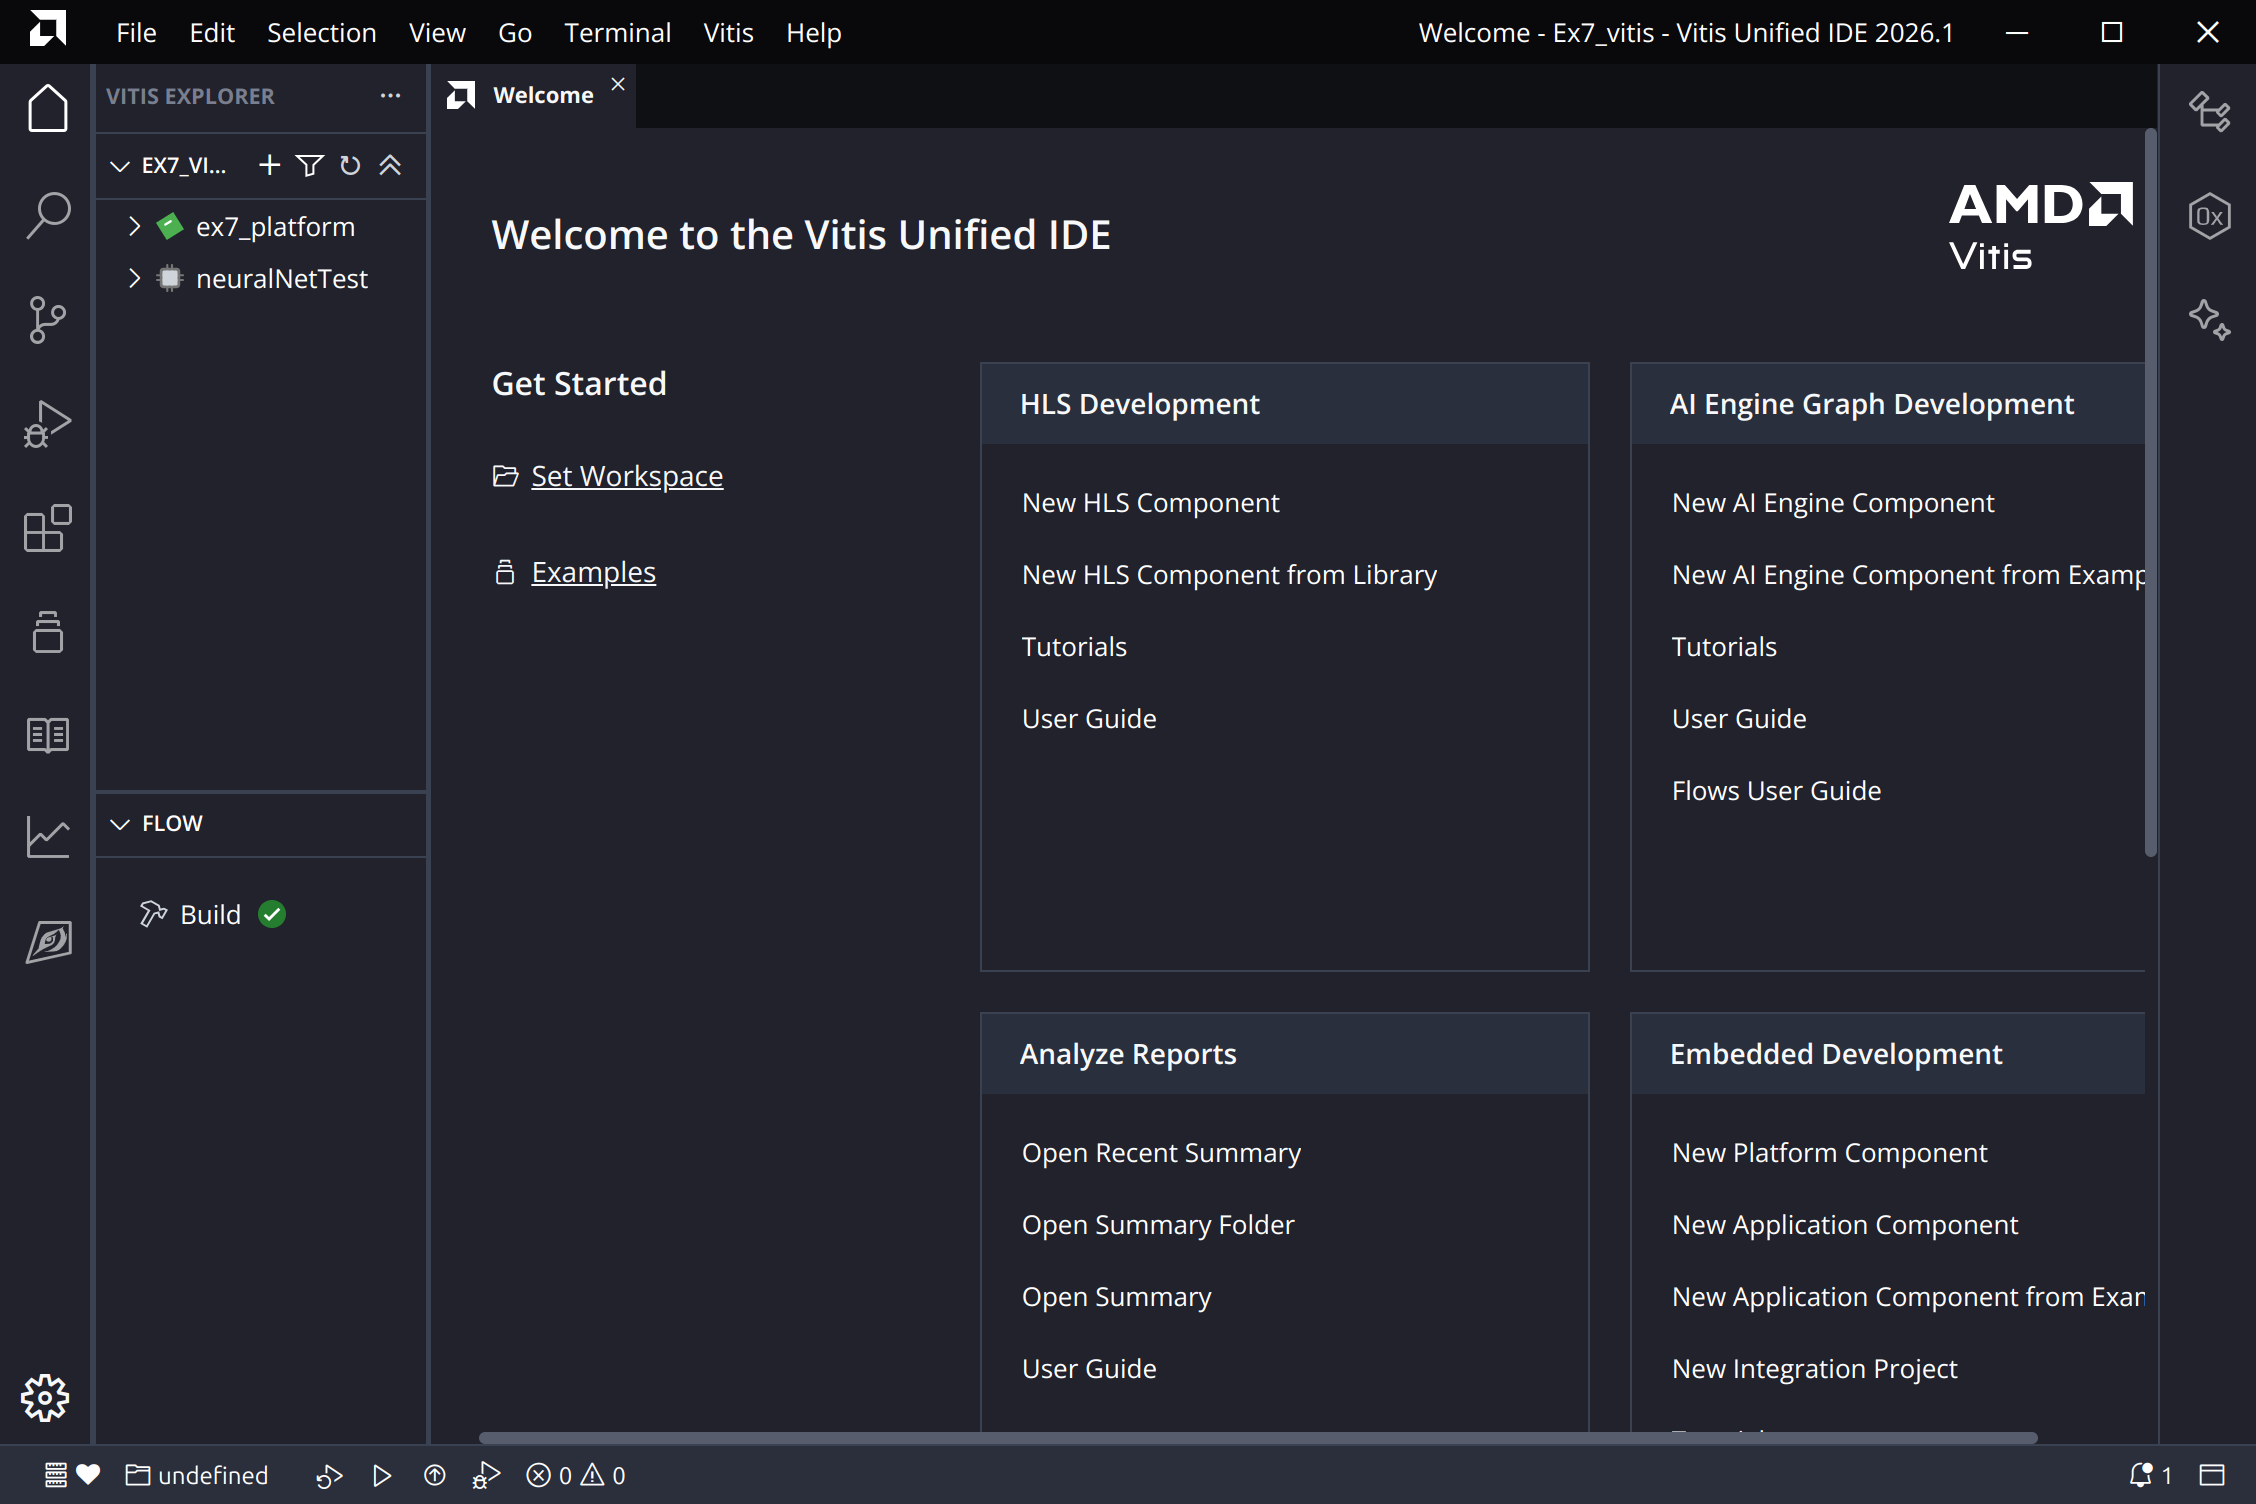
\includegraphics[width=\textwidth]{native_screenshots/vitis_neuralNetTest_maximized.png}
\caption{Historical native capture (10 October): Vitis 2026.1 application build}
\label{fig:vitis-build}
\end{figure}

The fresh ELF was downloaded with XSDB after programming the rebuilt bitstream
and initializing the processing system. Figure~\ref{fig:uart-run} preserves the
earlier UART screenshot; its timing values are historical and are superseded
by the fresh measurements above and raw transcript below.

\begin{figure}[H]
\centering
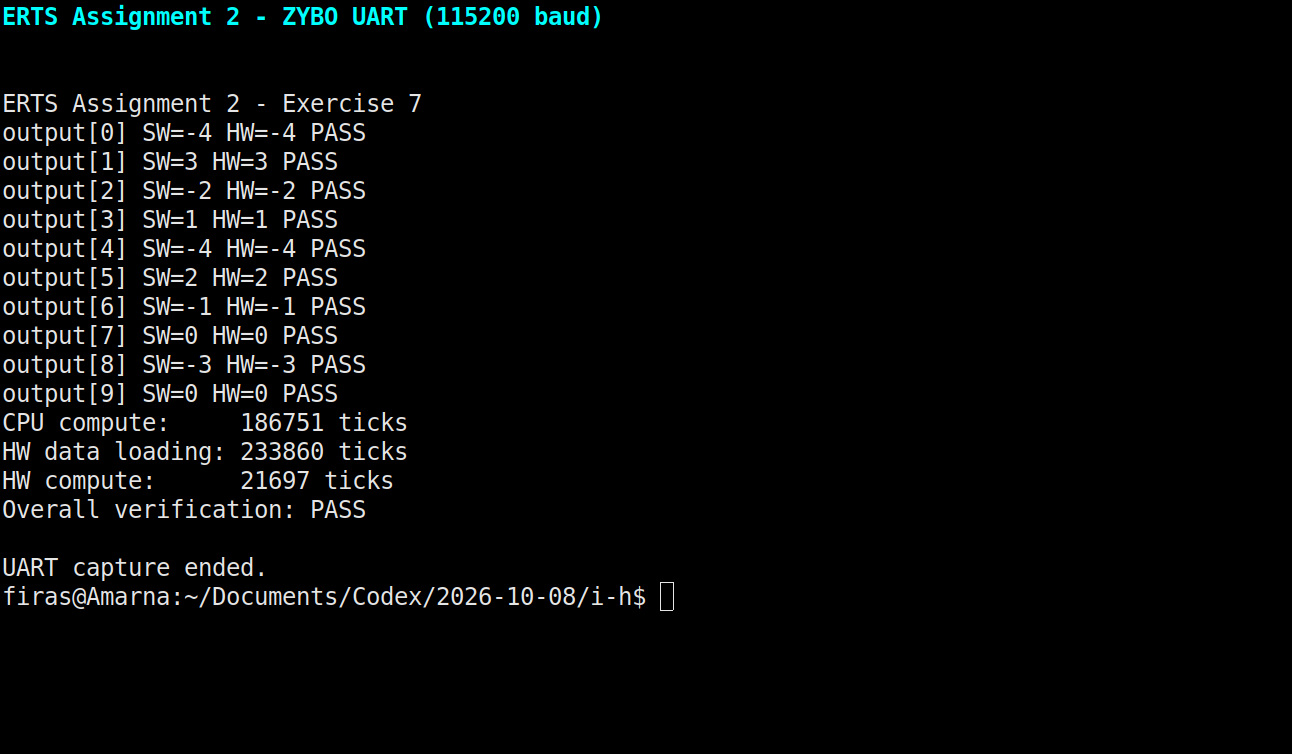
\includegraphics[width=\textwidth,trim=0 215 0 0,clip]{native_screenshots/ex7_board_uart_window.png}
\caption{Historical native capture (10 October): earlier ZYBO run, before the \texttt{-O2} benchmark revision}
\label{fig:uart-run}
\end{figure}

\subsection{Fresh Native UART Transcript}
The following is a typeset copy of the actual captured serial bytes from the
11 October post-fix run, not a screenshot or reconstructed terminal image.
Bitstream/ELF hashes are retained beside the log in \texttt{metadata.json}.
\lstinputlisting[style=cppstyle,language={},numbers=none,basicstyle=\ttfamily\footnotesize,caption={Actual post-fix ZYBO UART output}]{fix_evidence/board_ex7_20261011/uart.log}

\section{Conclusion}
The assignment demonstrates a progression from processor-only control to
hardware acceleration. Exercise 3 establishes UART, GPIO, and timer control.
Exercise 4 provides a verified software reference. Exercise 5 moves the inner
matrix operation into programmable logic and makes communication overhead
explicit. Exercise 7 applies the same method to a fixed-point neural network and
shows that targeted pipelining reduces latency substantially at moderate resource
cost.

The post-review code fixes address peripheral selection, on-chip memory,
course matrix interfaces, verification coverage and benchmark boundaries.
Exercises 3--5 have native builds and real UART results, and the user confirmed
the physical counter. The ANN uses a documented adapted reference rather than
claiming that the original supplied test passes. Tool-version/reference
acceptance and any unobserved switch/LED mapping remain explicit limitations.

\section*{Reproducibility}
\begin{itemize}[leftmargin=2em]
  \item Source branch: \texttt{assignment\_2/Firas}
  \item Hardware implementation commit: \texttt{29f6373}
  \item Native target-validation commit: \texttt{cbec41c}
  \item Pre-fix review snapshot: \texttt{c38a216}; this revision includes local post-review fixes.
  \item Target part: \texttt{xc7z010clg400-1}
  \item HLS target clock: 10 ns
  \item Matrix test: \texttt{make -C Assignment\_2 test}
  \item HLS flow: \texttt{vitis-run --mode hls --tcl run\_hls.tcl}
  \item Vitis application: \texttt{vitis -s build\_vitis\_2026.py}
  \item Fresh build/UART logs and artifact hashes: \path{outputs/fix_evidence/}
  \item Three native apps and OCM proof: \path{Assignment_2/hardware/Ex345_vitis/}
\end{itemize}

\appendix
\section{Source File Map}
\begin{table}[H]
\centering
\scriptsize
\begin{tabularx}{\textwidth}{p{1.4cm} >{\raggedright\arraybackslash}p{7.2cm} >{\raggedright\arraybackslash}X}
\toprule
\textbf{Exercise} & \textbf{Source location} & \textbf{Primary contents} \\
\midrule
3 & \path{Assignment_2/exercise3_console/src/main.c} & UART, GPIO, counter \\
4 & \path{Assignment_2/exercise4_matrix/src/main.c} & Software command and timing \\
4, 5 & \path{Assignment_2/common/matrix.c} & Matrices and reference multiply \\
5 & \path{Assignment_2/exercise5_matrix_ip/src/main.c} & AXI benchmark \\
7 & \path{Assignment_2/exercise7_neural_net/hls/neuralNet.cpp} & Synthesizable ANN \\
7 & \path{Assignment_2/exercise7_neural_net/hls/testbench.cpp} & Self-checking model \\
7 & \path{Assignment_2/exercise7_neural_net/hls/run_hls.tcl} & HLS solutions \\
7 & \path{Assignment_2/exercise7_neural_net/sdk/neuralNetTest.c} & Target benchmark \\
\bottomrule
\end{tabularx}
\end{table}

\end{document}
